\chapter{Specifikacija programske potpore}
		
	\section{Funkcionalni zahtjevi}
			
			\noindent \textbf{Dionici:}
			
			\begin{packed_enum}
				
				\item Vlasnik (naručitelj)
				\item Članovi organizacije
				
				\begin{packed_enum}
					\item Zaposlenik
					\item Revizor
					\item Računovođa
					\item Direktor
				\end{packed_enum}
				
				\item Administrator
				\item Razvojni tim
				
			\end{packed_enum}
			
			\noindent \textbf{Aktori i njihovi funkcionalni zahtjevi:}
			
			
			\begin{packed_enum}
				
				\item  \underbar{Neregistrirani/neprijavljeni korisnik (inicijator) može:}
				\begin{packed_enum}
					
					\item se prijaviti u sustav pomoću kredencijala (e-mail adresa i lozinka) koje je dobio od superriornije osobe 
					
				\end{packed_enum}
			
				\item  \underbar{Zaposlenik (inicijator) može:}
				\begin{packed_enum}
					
					\item prijaviti se u sustav
					\item pregledati svoje osobne podatke (ime, prezime, nadređeni revizor)
					\item skenirati dokumente koje se spremaju u njegovu internu bazu
					\item potvrditi dokumente koje je prethodno skenirao
					\item primiti obavijesti od revizora i nadređenih zaposlenika tvrtke
					\item poslati revizirane dokumente od njegove strane na dodatan pregled
					\item vidjeti svoju internu bazu prethodno skeniranih dokumenata
					
				\end{packed_enum}
				
				\item  \underbar{Revizor (inicijator) može:}
				\begin{packed_enum}
					
					\item prijaviti se u sustav
					\item pregledati svoje osobne podatke (ime, prezime, popis podređenih zaposlenika)
					\item dobiti obavijesti o skeniranim dokumentima od strane podređenog zaposlenika
					\item skenirati dokumente koje se spremaju u njegovu internu bazu
					\item revizirati primljene dokumente
					\item proslijediti određenom računovođi dokument skeniran i potvrđen od strane podređenog zaposlenika
					
				\end{packed_enum}
				
				\item  \underbar{Računovođa (inicijator) može:}
				\begin{packed_enum}
					
					\item prijaviti se u sustav
					\item pregledati svoje osobne podatke (ime, prezime, vrstu dokumenta za koju je zaslužan)
					\item pregledati dokumente spremne za arhiviranje
					\item arhivirati dokumente
					\item pregledati povijest dokumenata koje je arhivirao u svojoj internoj bazi
					\item prosljediti dokumente direktoru na potpis prije arhiviranja
					
				\end{packed_enum}
				
				\item  \underbar{Direktor (inicijator) može:}
				\begin{packed_enum}
					
					\item prijaviti se u sustav
					\item pregledati svoje osobne podatke (ime, prezime, ime tvrtke za koju je zaslužan)
					\item primati obavijesti o zatraženim potpisima o računovođi
					\item pregledati popis svih korisnika aplikacije
					\item pregledati statistike zaposlenika (broj skeniranih dokumenata,
					prosjek skeniranih dokumenata svih zaposlenika te ostale statistike)
					\item promjeniti uloge i ostale podatke o svim ostalim korisnicima unutar tvrtke 
					\item brisati račune otpuštenih zaposlenika tvrtke te ih također stvarati
					\item pregledati sve dokumente i njihovu povijest(tko ih je skenirao, 
					revizirao i koji računovođa je bio zaslužan za njihovo arhiviranje)
					\item objaviti određeni dokument na društvenim mrežama
					
				\end{packed_enum}
				
				\item  \underbar{Administrator (inicijator) može:}
				\begin{packed_enum}
					
					\item prijaviti se u sustav
					\item dodavati različite tvrtke i njihove direktore
					\item pregledati osobne podatke svih korisnika aplikacije
					
					%\item upozoravati direktora na kršenje uvijete poslovanja aplikacije
					%\item brisati korisnika koji krše uvijete poslovanja aplikacije
					
				\end{packed_enum}
				
				\clearpage
				
				\item  \underbar{Baza podataka (sudionik) može:}
				\begin{packed_enum}
					
					\item pohraniti podatke o svim korisnicima aplikacije
					\item pohraniti sve podatke o tvrtkama te arhivitra sve dokumente određene tvrtke
					
				\end{packed_enum}
				
				
			\end{packed_enum}
			
			\eject 
			
			
				
			\subsection{Obrasci uporabe}
							
				\subsubsection{Opis obrazaca uporabe}


					\noindent \underbar{\textbf{UC1 -Registracija u sustav}}
					\begin{packed_item}
	
						\item \textbf{Glavni sudionik: }Direktor, Administrator
						\item  \textbf{Cilj:} Stvoriti korisnički račun za pristup sustavu
						\item  \textbf{Sudionici:} Baza podataka
						\item  \textbf{Preduvjet:} -
						\item  \textbf{Opis osnovnog tijeka:}
						
						\item[] \begin{packed_enum}
	
							\item Aktor odabire opciju za registraciju
							\item Aktor unosi osobne podatke za novog korisnika
							\item Šalje se mail novododanom korisniku s njegovim podacima za prijavu
						\end{packed_enum}
						
						\item  \textbf{Opis mogućih odstupanja:}
						
						\item[] \begin{packed_item}
	
							\item[2.a] Korisnik je već registriran u sustav
							\item[] \begin{packed_enum}
								
								\item Sustav daje audio-vizualnu obavjest aktoru da je korisnik već registriran
								
							\end{packed_enum}
							
							\item[2.b] Neispravna e-mail adresa
							\item[] \begin{packed_enum}
								
								\item Sustav daje auditornu i vizualnu obavjest aktoru da je e-mail adresa neispravna
								\item Aktor upisuje ispravnu e-mail adresu
							\end{packed_enum}
							
						\end{packed_item}
					\end{packed_item}
					
					
					\noindent \underbar{\textbf{UC2 -Prijava u sustav}}
					\begin{packed_item}
						
						\item \textbf{Glavni sudionik: }članovi organizacije, Administrator
						\item  \textbf{Cilj:} Prijava za pristup funkcionalnost aplikacije
						\item  \textbf{Sudionici:} Baza podataka
						\item  \textbf{Preduvjet:} Aktor je registriran
						\item  \textbf{Opis osnovnog tijeka:}
						
						\item[] \begin{packed_enum}
							
							\item Aktor unosi svoje osobne podatke
							\item Sustav provjerava jesu li podnešeni podaci ispravni
							\item Aktor biva prijavljen u aplikaciju
						\end{packed_enum}
						
						\item  \textbf{Opis mogućih odstupanja:}
						
						\item[] \begin{packed_item}
							
							\item[2.a] Unešeni osobni podaci ne odgovaraju niti jednom registriranom korisniku
							\item[] \begin{packed_enum}
								
								\item Sustav daje audio-vizualnu obavjest aktoru da su osobni podaci neispravni
								\item Sustav daje priliku aktoru za ponovnu prijavu
								
							\end{packed_enum}
							
						\end{packed_item}
					\end{packed_item}
				
				
					\noindent \underbar{\textbf{UC3 -Brisanje korisnika iz sustava}}
					\begin{packed_item}
						
						\item \textbf{Glavni sudionik: }Direktor, Administrator
						\item  \textbf{Cilj:} Brisanje korisničkog računa
						\item  \textbf{Sudionici:} Baza podataka
						\item  \textbf{Preduvjet:} Korisnik računa je registriran u sustav
						\item  \textbf{Opis osnovnog tijeka:}
						
						\item[] \begin{packed_enum}
							
							\item Aktor otvara administrativnu ploču
							\item Aktor odabire popis svih registriranih klijenata
							\item Aktor odabire korisnika kojeg želi izbrisati
							\item Aktor briše korisnika
							\item Baza podataka briše račun korisnika
							\item Aktora se vraća na popis svih registriranih klijenata
							\end{packed_enum}
						
					\end{packed_item}
					
					\noindent \underbar{\textbf{UC4 -Pregled korisničkih podataka}}
					\begin{packed_item}
						
						\item \textbf{Glavni sudionik: }Direktor, Administrator
						\item  \textbf{Cilj:} Dobiti uvid u osobne podatke klijenta
						\item  \textbf{Sudionici:} Baza podataka
						\item  \textbf{Preduvjet:} Prijavljen
						\item  \textbf{Opis osnovnog tijeka:}
						
						\item[] \begin{packed_enum}
							
							\item Aktor otvara listu svih korisnika
							\item Baza podataka dohvaća listu svih registriranih korisnika
							\item Aktor odabire određenog korisnika na danom popisu
							\item Baza podataka dohvaća osobne podatke odabranog korisnika
						
						\end{packed_enum}
						
					\end{packed_item}
					
					
					\noindent \underbar{\textbf{UC5 -Promjena podataka zaposlenika}}
					\begin{packed_item}
						
						\item \textbf{Glavni sudionik: }Direktor
						\item  \textbf{Cilj:} Napraviti promjena nad osobnim podatcima zaposlenika tvrtke
						\item  \textbf{Sudionici:} Baza podataka
						\item  \textbf{Preduvjet:} Prijavljen u sustav
						\item  \textbf{Opis osnovnog tijeka:}
						
						\item[] \begin{packed_enum}
							
							\item Direktor je odabrao opciju za prikaz svih zaposlenika tvrtke
							\item Baza dohvaća popis svih zaposlenika tvrtke
							\item Direktor odabire određenog zaposlenika
							\item Baza podataka dohvaća odabranog zaposlenika
							\item Direktoru se prikazuju podatci zaposlenika
							\item Direktor mijenja njegove podatke
							\item Direktor sprema podatke pritiskom na tipku
							\item Baza podataka sprema nove promijene nad zaposlenikom
						 
						\end{packed_enum}
						
						\item  \textbf{Opis mogućih odstupanja:}
						
						\item[] \begin{packed_item}
							
							\item[7.a] Direktor nije odabrao  opciju spremanja podataka prije izlaska iz sučelja
							\item[] \begin{packed_enum}
								
								\item Sustav daje audio-vizualnu obavjest direktoru da se promijenjeni podatci neće spremiti
								\item Direktor odabire želi li odbaciti/spremiti novo nastale promijene
								
							\end{packed_enum}
							
							\item[7.b] Direktor je unio nove neispravne podatke
							\item[] \begin{packed_enum}
								
								\item Sustav daje auditornu i vizualnu obavjest direktoru da su određeni podatci neispravni
								\item Direktor odabire  želi li promijeniti ili odbaciiti neispravne podatke
								
							\end{packed_enum}
							
						\end{packed_item}
					\end{packed_item}
					
										
					\noindent \underbar{\textbf{UC6 - Primanje obavijesti}}
					\begin{packed_item}
						
						\item \textbf{Glavni sudionik: } Zaposlenik, Revizor, Računovođa, Direktor
						\item \textbf{Cilj:} Primiti obavijesti od aplikacije
						\item \textbf{Sudionici:} Aplikacija
						\item \textbf{Preduvjet:} Prijavljen u sustav
						\item \textbf{Opis osnovnog tijeka:}
						
						\item[] \begin{packed_enum}
							
							\item Aplikacija šalje obavijesti korisniku o relevantnim događajima ili zadacima
							\item Korisnik prima obavijesti putem aplikacije ili e-pošte
							
						\end{packed_enum}
					\end{packed_item}
					
					
					\noindent \underbar{\textbf{UC7 - Pregledavanje statistike zaposlenika tvrtke}}
					\begin{packed_item}
						
						\item \textbf{Glavni sudionik: } Direktor
						\item \textbf{Cilj:} Pregledati statističke podatke o zaposlenicima tvrtke
						\item \textbf{Sudionici:} Baza podataka
						\item \textbf{Preduvjet:} Prijavljen u sustav
						\item \textbf{Opis osnovnog tijeka:}
						
						\item[] \begin{packed_enum}
							
							\item Direktor otvara statističku sekciju aplikacije
							\item Sustav dohvaća statističke podatke o zaposlenicima
							\item Direktor pregledava informacije o radu i aktivnostima zaposlenika
							
						\end{packed_enum}
					\end{packed_item}
					
					
					\noindent \underbar{\textbf{UC8 - Pregled svih dokumenata}}
					\begin{packed_item}
						
						\item \textbf{Glavni sudionik: } Direktor
						\item \textbf{Cilj:} Pregledati sve dokumente
						\item \textbf{Sudionici:} Baza podataka
						\item \textbf{Preduvjet:} Prijavljen u sustav
						\item \textbf{Opis osnovnog tijeka:}
						
						\item[] \begin{packed_enum}
							
							\item Direktor odabire pregled popisa svih dokumenata
							\item Sustav prikazuje popis svih dokumenata
							\item Direktor pregledava dokumente i njihove detalje
							
						\end{packed_enum}
					\end{packed_item}
					
					
					\noindent \underbar{\textbf{UC9 - Pregled skeniranih dokumenata}}
					\begin{packed_item}
						
						\item \textbf{Glavni sudionik: } Zaposlenik, Revizor, Računovođa, Direktor
						\item \textbf{Cilj:} Pregledati skenirane dokumente
						\item \textbf{Sudionici:} Baza podataka
						\item \textbf{Preduvjet:} Prijavljen u sustav
						\item \textbf{Opis osnovnog tijeka:}
						
						\item[] \begin{packed_enum}
							
							\item Aktor odabire pregled popisa svih dokumenata koje je skenirao
							\item Sustav prikazuje popis svih dokumenata skeniranih od strane aktora
							\item Aktor pregledava dokumente i njihove detalje
							
						\end{packed_enum}
					\end{packed_item}
					
					
					\noindent \underbar{\textbf{UC10 - Pregled dokumenata spremnih za reviziranje}}
					\begin{packed_item}
						
						\item \textbf{Glavni sudionik: } Revizor
						\item \textbf{Cilj:} Pregledati dokumente spremne za reviziranje
						\item \textbf{Sudionici:} Baza podataka
						\item \textbf{Preduvjet:} Prijavljen u sustav
						\item \textbf{Opis osnovnog tijeka:}
						
						\item[] \begin{packed_enum}
							
							\item Revizor odabire pregled popisa svih dokumenata koje je skenirao
							\item Sustav prikazuje popis svih dokumenata spremnih za reviziranje
							\item Revizor pregledava dokumente spremne za reviziranje i njihove detalje
							
						\end{packed_enum}
					\end{packed_item}
					
										
					\noindent \underbar{\textbf{UC11 - Pregled dokumenata spremnih za arhiviranje}}
					\begin{packed_item}
						
						\item \textbf{Glavni sudionik: } Računovođa
						\item \textbf{Cilj:} Pregledati dokumente spremne za arhiviranje
						\item \textbf{Sudionici:} Baza podataka
						\item \textbf{Preduvjet:} Prijavljen u sustav
						\item \textbf{Opis osnovnog tijeka:}
						
						\item[] \begin{packed_enum}
							
							\item Računovođa odabire pregled popisa svih dokumenata spremnih za arhiviranje
							\item Sustav prikazuje popis svih dokumenata spremnih za arhiviranje
							\item Računovođa pregledava dokumente spremne za arhiviranje i njihove detalje
							
						\end{packed_enum}
					\end{packed_item}
					
					
					\noindent \underbar{\textbf{UC12 - Pregled dokumenata koji čekaju potpis}}
					\begin{packed_item}
						
						\item \textbf{Glavni sudionik: } Računovođa, Direktor
						\item \textbf{Cilj:} Pregledati dokumente za koje je potreban potpis
						\item \textbf{Sudionici:} Baza podataka
						\item \textbf{Preduvjet:} Prijavljen u sustav
						\item \textbf{Opis osnovnog tijeka:}
						
						\item[] \begin{packed_enum}
							
							\item Računovođa odabire pregled popisa svih dokumenata za koje je potreban potpis
							\item Sustav prikazuje popis svih dokumenata za koje je potreban potpis
							\item Računovođa pregledava dokumente spremne za koje je potreban potpis i njihove detalje
							
						\end{packed_enum}
					\end{packed_item}
					
					
					\noindent \underbar{\textbf{UC13 - Pregled svih arhiviranih dokumenata određenog tipa}}
					\begin{packed_item}
						
						\item \textbf{Glavni sudionik: } Računovođa
						\item \textbf{Cilj:} Pregledati sve arhivirane dokumente za čiji je tip zaslužan
						\item \textbf{Sudionici:} Baza podataka
						\item \textbf{Preduvjet:} Prijavljen u sustav
						\item \textbf{Opis osnovnog tijeka:}
						
						\item[] \begin{packed_enum}
							
							\item Računovođa odabire pregled popisa svih arhiviranih dokumenata za čiji je tip zaslužan
							\item Sustav prikazuje popis svih takvih dokumenata
							\item Računovođa pregledava arhivirane dokumente
							
						\end{packed_enum}
					\end{packed_item}
					
					
					\noindent \underbar{\textbf{UC14 - Pregled svih reziviranih dokumenata određenog tipa}}
					\begin{packed_item}
						
						\item \textbf{Glavni sudionik: } Računovođa
						\item \textbf{Cilj:} Pregledati sve revizirane dokumente za čiji je tip zaslužan
						\item \textbf{Sudionici:} Baza podataka
						\item \textbf{Preduvjet:} Prijavljen u sustav
						\item \textbf{Opis osnovnog tijeka:}
						
						\item[] \begin{packed_enum}
							
							\item Računovođa odabire pregled popisa svih reviziranih dokumenata za čiji je tip zaslužan
							\item Sustav prikazuje popis svih takvih dokumenata
							\item Računovođa pregledava revizirane dokumente
							
						\end{packed_enum}
					\end{packed_item}
					
					
					\noindent \underbar{\textbf{UC15 - Objava dokumenta na društvene mreže}}
					\begin{packed_item}
						
						\item \textbf{Glavni sudionik: } Direktor
						\item \textbf{Cilj:} Objaviti odabrani dokument na društvenim mrežama
						\item \textbf{Sudionici:} Društvene mreže, Baza podataka
						\item \textbf{Preduvjet:} Prijavljen u sustav
						\item \textbf{Opis osnovnog tijeka:}
						
						\item[] \begin{packed_enum}
							
							\item Direktor odabire opciju za prikaz popisa svih dokumenata tvrtke
							\item Direktor odabire dokument koji želi podijeliti na društvenim mrežama
							\item Sustav omogućuje izbor društvenih mreža za objavu
							\item Direktor potvrđuje i dijeli dokument na odabranim društvenim mrežama
							
						\end{packed_enum}
					\end{packed_item}
					
					
					\noindent \underbar{\textbf{UC16 - Pregledavanje dokumenata s liste}}
					\begin{packed_item}
						
						\item \textbf{Glavni sudionik: } Zaposlenik, Revizor, Računovođa, Direktor
						\item \textbf{Cilj:} Pregledati dostupne dokumente
						\item \textbf{Sudionici:} Baza podataka
						\item \textbf{Preduvjet:} Prijavljen u sustav
						\item \textbf{Opis osnovnog tijeka:}
						
						\item[] \begin{packed_enum}
							
							\item Aktor odabire neku od opcija za prikaz liste dokumenata
							\item Sustav prikazuje popis dostupnih dokumenata
							\item Aktor odabire dokument za pregled
							\item Sustav prikazuje detalje odabranog dokumenta
							
						\end{packed_enum}
					\end{packed_item}
					
					
					\noindent \underbar{\textbf{UC17 - Arhiviranje dokumenata}}
					\begin{packed_item}
						
						\item \textbf{Glavni sudionik: } Računovođa
						\item \textbf{Cilj:} Arhivirati odabrane dokumente
						\item \textbf{Sudionici:} Baza podataka
						\item \textbf{Preduvjet:} Prijavljen u sustav
						\item \textbf{Opis osnovnog tijeka:}
						
						\item[] \begin{packed_enum}
							
							\item Računovođa otvara listu potpisanih dokumenata ili listu dokumenata spremnih za arhiviranje
							\item Računovođa odabire dokumente koje želi arhivirati
							\item Sustav omogućuje odabir mjesta za arhiviranje
							\item Računovođa potvrđuje i arhivira dokumente
							
						\end{packed_enum}
					\end{packed_item}
					
					
					\noindent \underbar{\textbf{UC18 - Potpisivanje dokumenata}}
					\begin{packed_item}
						
						\item \textbf{Glavni sudionik: } Direktor
						\item \textbf{Cilj:} Potpisati odabrane dokumente prije njihovog arhiviranja
						\item \textbf{Sudionici:} Baza podataka
						\item \textbf{Preduvjet:} Prijavljen u sustav
						\item \textbf{Opis osnovnog tijeka:}
						
						\item[] \begin{packed_enum}
							
							\item Direktor odabire opciju za prikaz dokumenata koji čekaju potpis
							\item Direktor odabire dokumente koje želi potpisati
							\item Sustav omogućuje pregled odabranih dokumenata
							\item Nadležni direktor potpisuje dokumente
							
						\end{packed_enum}
					\end{packed_item}
					
					
					\noindent \underbar{\textbf{UC19 - Slanje dokumenta na potpis}}
					\begin{packed_item}
						
						\item \textbf{Glavni sudionik: } Računovođa
						\item \textbf{Cilj:} Poslati odabrani dokument na potpis nadležnom direktoru
						\item \textbf{Sudionici:} Baza podataka
						\item \textbf{Preduvjet:} Prijavljen u sustav
						\item \textbf{Opis osnovnog tijeka:}
						
						\item[] \begin{packed_enum}
							
							\item Računovođa odabire opciju za prikaz dokumenata koji čekaju arhiviranje
							\item Računovođa odabire dokument koji želi poslati na potpis
							\item Dokument se šalje na potpis nadležnom direktoru
							\item Nadležni direktor prima obavijest o dokumentu za potpis
							
						\end{packed_enum}
					\end{packed_item}
					
					
					\noindent \underbar{\textbf{UC20 - Učitavanje slika dokumenata}}
					\begin{packed_item}
						
						\item \textbf{Glavni sudionik: } Zaposlenik, Revizor, Računovođa, Direktor
						\item \textbf{Cilj:} Učitavanje slika dokumenata za digitalizaciju
						\item \textbf{Sudionici:} Baza podataka
						\item \textbf{Preduvjet:} Prijavljen u sustav
						\item \textbf{Opis osnovnog tijeka:}
						
						\item[] \begin{packed_enum}
							
							\item Aktor odabire opciju za učitavanje slika dokumenata
							\item Aktor odabire do 50 slika za učitavanje
							\item Sustav šalje slike na OCR
							
						\end{packed_enum}
						
						\item \textbf{Opis mogućih odstupanja:}
						
						\item[] \begin{packed_item}
							
							\item[2.a] Aktor odabire više od 50 slika za učitavanje
							\item[] \begin{packed_enum}
								
								\item Sustav daje audio-vizualnu obavijest korisniku da je premašen maksimalni broj slika
								\item Aktor odabire do 50 slika za učitavanje
								
							\end{packed_enum}
							
						\end{packed_item}
					\end{packed_item}
					
					
					\noindent \underbar{\textbf{UC21 - Digitializacija dokumenta}}
					\begin{packed_item}
						
						\item \textbf{Glavni sudionik: } Sustav
						\item \textbf{Cilj:} Detektirati dokument sa učitane slike te ga pretvoriti u digitalni oblik
						\item \textbf{Sudionici:} Baza podataka
						\item \textbf{Preduvjet:} Dokument je uslikan
						\item \textbf{Opis osnovnog tijeka:}
						
						\item[] \begin{packed_enum}
							
							\item Sustav učitava sliku primljenu na danju obradu od strane aktora
							\item Sustav pregledava danu sliku te utvrđuje nalazi li se dokument na slici
							\item Sustav primjenjuje OCR na detektirani dokument na slici
							\item Sustav sprema novonastali dokument u bazu podataka
							
						\end{packed_enum}
						
						\item \textbf{Opis mogućih odstupanja:}
						
						\item[] \begin{packed_item}
							
							\item[2.a] Sustav nije pronašao dokument na slici
							\item[] \begin{packed_enum}
								
								\item Sustav daje audio-vizualnu obavijest aktoru da učitana slika ne sadrži dokument
								\item Sustav daje opciju aktoru da priloži drugu sliku ili da odustane od daljnje obrade
								
							\end{packed_enum}
							
						\end{packed_item}
						
					\end{packed_item}
					
				\clearpage
					
				\subsubsection{Dijagrami obrazaca uporabe}
					
					\begin{figure}[H]
						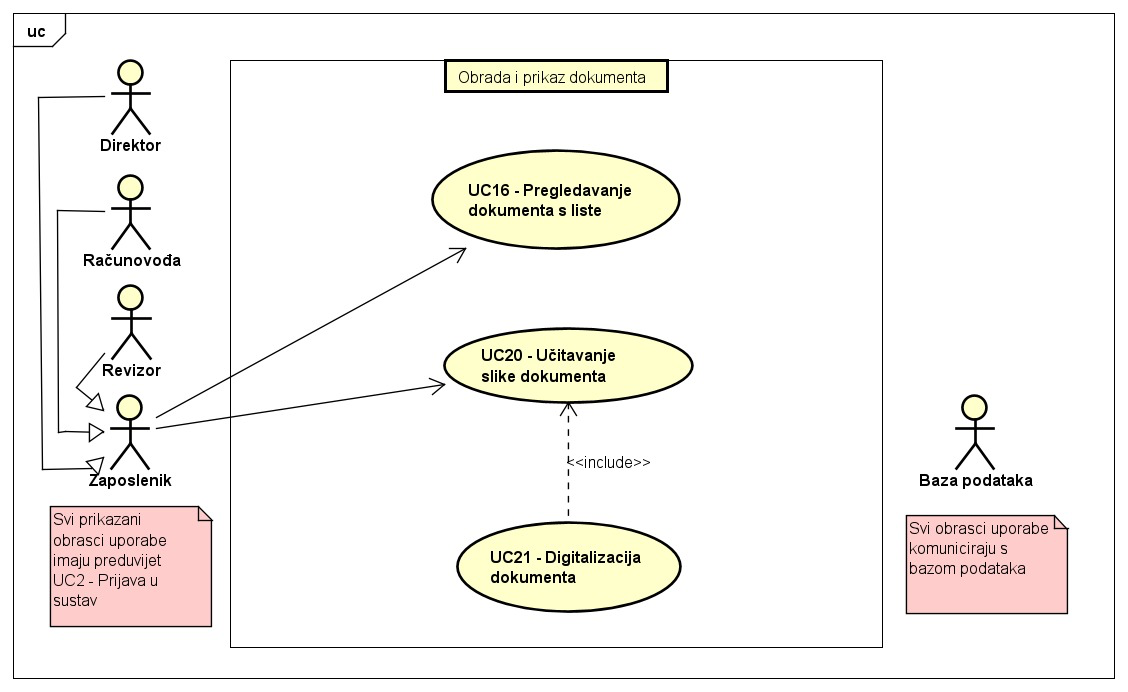
\includegraphics[width=\textwidth]{slike/3.1.1 dijagrami/ObradaIPrikazDokumenata.PNG}
						\caption{Dijagram obrasca uporabe, funkcionalnost svih aktora}
						\label{Obrazac1} 
					\end{figure}
					
					\begin{figure}[H]
						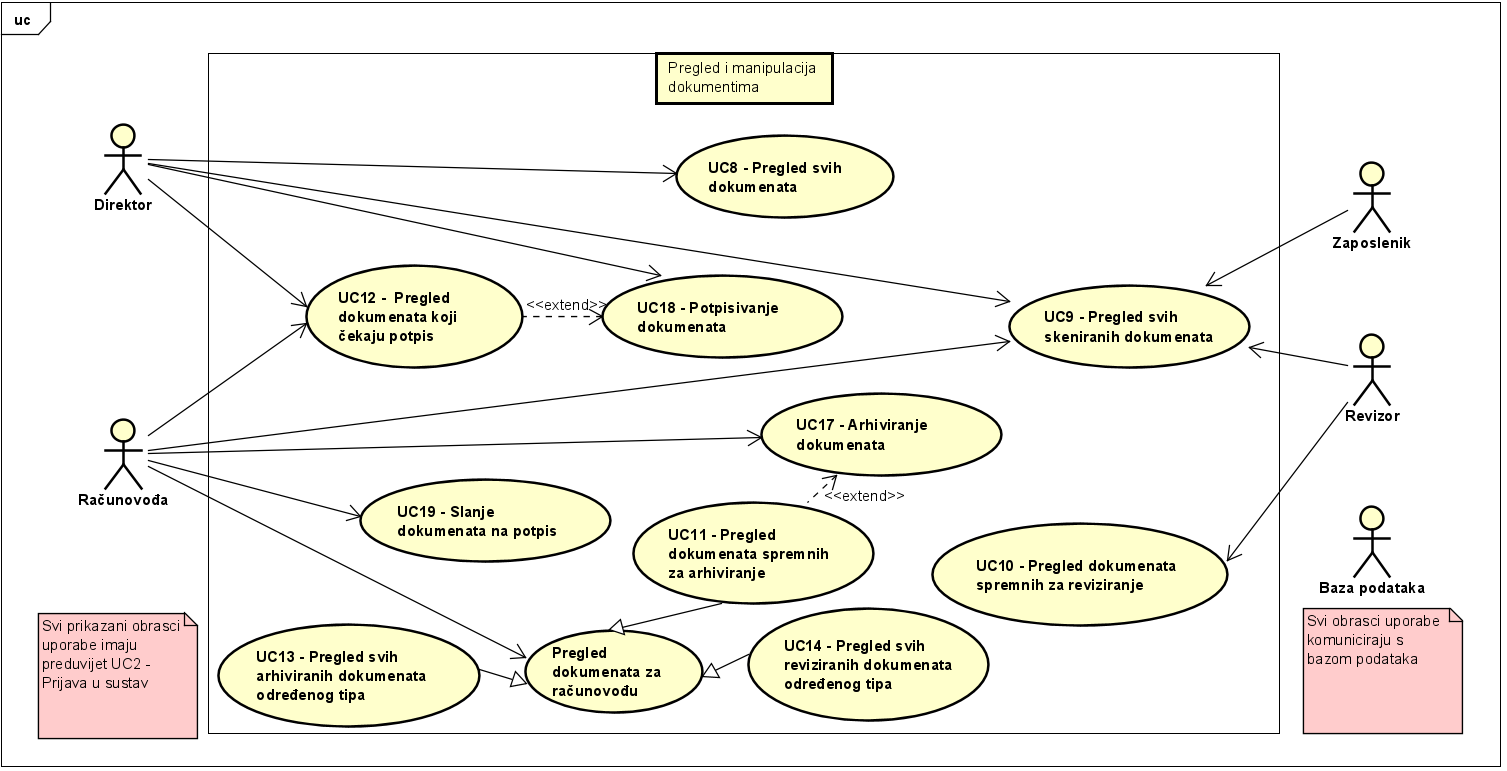
\includegraphics[width=\textwidth]{slike/3.1.1 dijagrami/PregledIManipulacijaDokumentima_v2.PNG}
						\caption{Dijagram obrasca uporabe, funkcionalnost svih aktora}
						\label{Obrazac2} 
					\end{figure}
					
					\begin{figure}[H]
						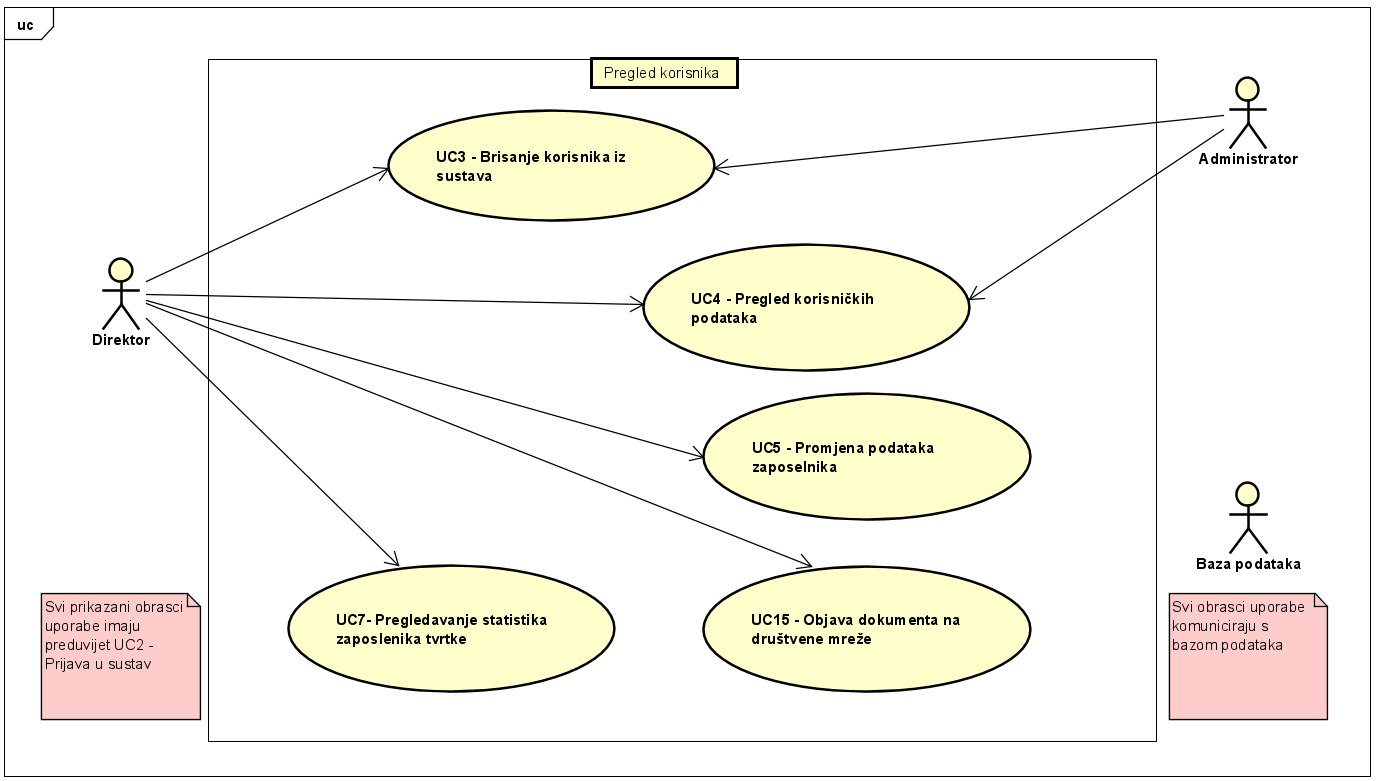
\includegraphics[width=\textwidth]{slike/3.1.1 dijagrami/PregledKorisnika.PNG}
						\caption{Dijagram obrasca uporabe, funkcionalnost Direktora i Administratora}
						\label{Obrazac3} 
					\end{figure}
					
					\begin{figure}[H]
						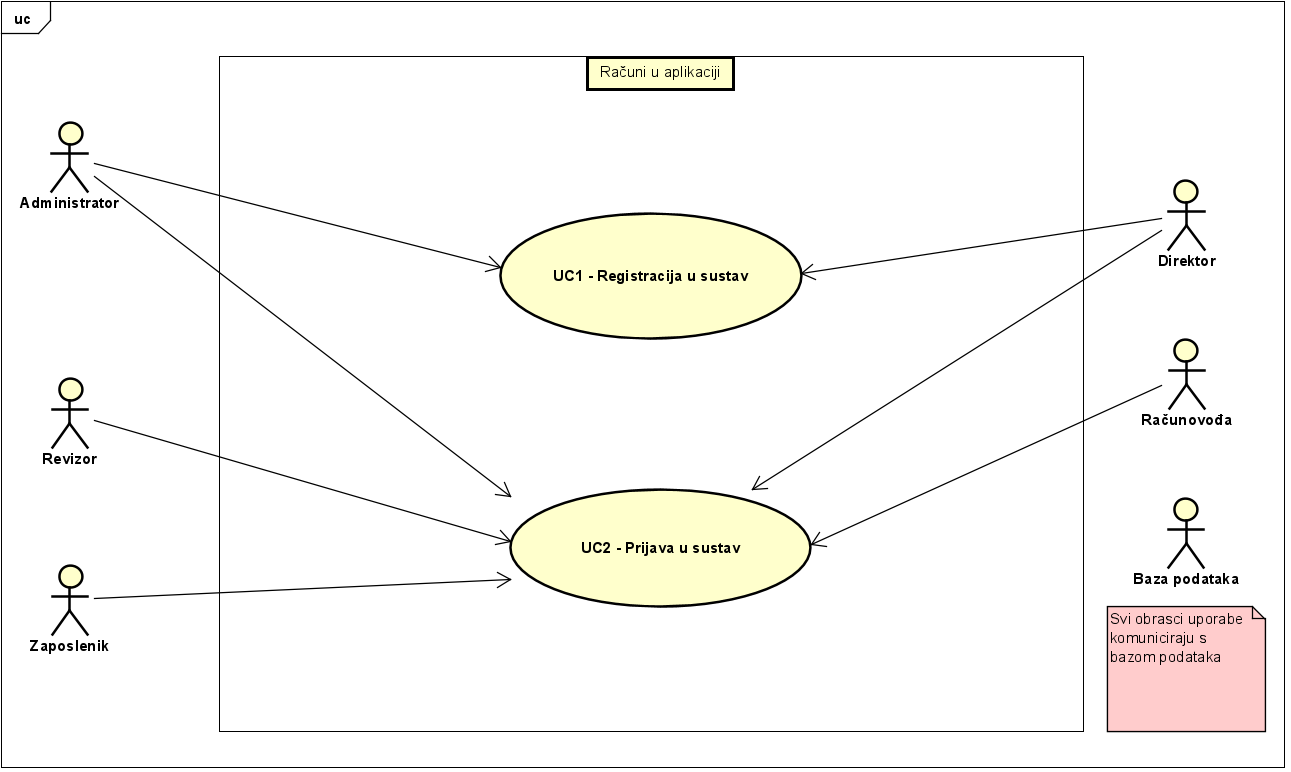
\includegraphics[width=\textwidth]{slike/3.1.1 dijagrami/RačuniUAplikaciji.PNG}
						\caption{Dijagram obrasca uporabe, funkcionalnost svih aktora}
						\label{Obrazac4} 
					\end{figure}
					
				\eject		
				
			\subsection{Sekvencijski dijagrami}
				
				\textbf{Obrazac uporabe UC2 - Prijava u sustav}\
				
				Korisnik unosi svoje osobne podatke. Sustav provjerava u bazi podataka jesu li uneseni podaci ispravni. Ako jesu, korisnik se prijavi u sustav. No ako uneseni podaci ne odgovaraju niti jednom registriranom korisniku u bazi, sustav korisniku šalje obavijest da su osobni podaci neispravni i daje mu priliku za ponovnu prijavu.
				\begin{figure}[H]
					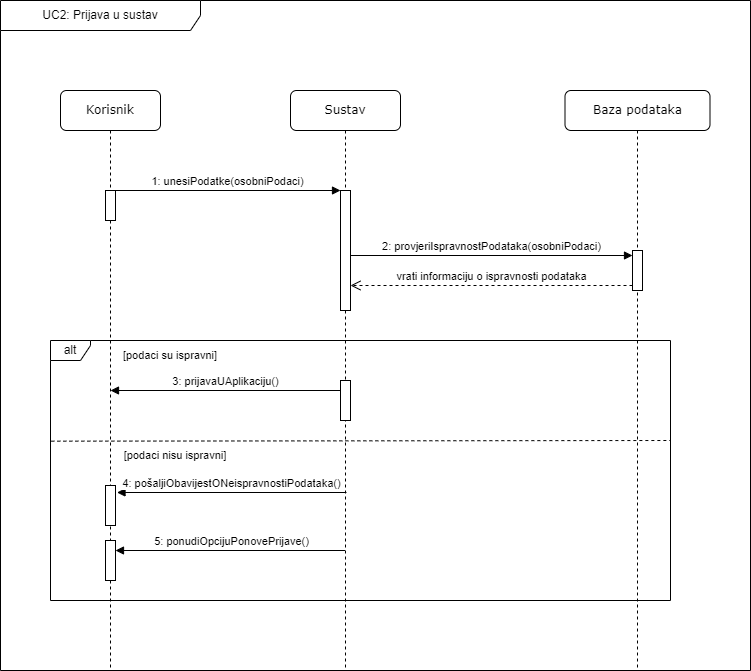
\includegraphics[width=\textwidth]{slike/sekvencijski_dijagram_UC2.PNG} %veličina u odnosu na širinu linije
					\caption{Slika broj: Sekvencijski dijagram za UC2}
					\label{fig:UC2} %label mora biti drugaciji za svaku sliku
				\end{figure}
				\clearpage

				\textbf{Obrazac uporabe UC9 - Pregled skeniranih dokumenata}\
				
				Korisnik odabire pregled popisa svih dokumenata koje je skenirao. Sustav pretraži u bazi njegove skenirane dokumente i vraća ih korisniku na uvid.
				\begin{figure}[H]
					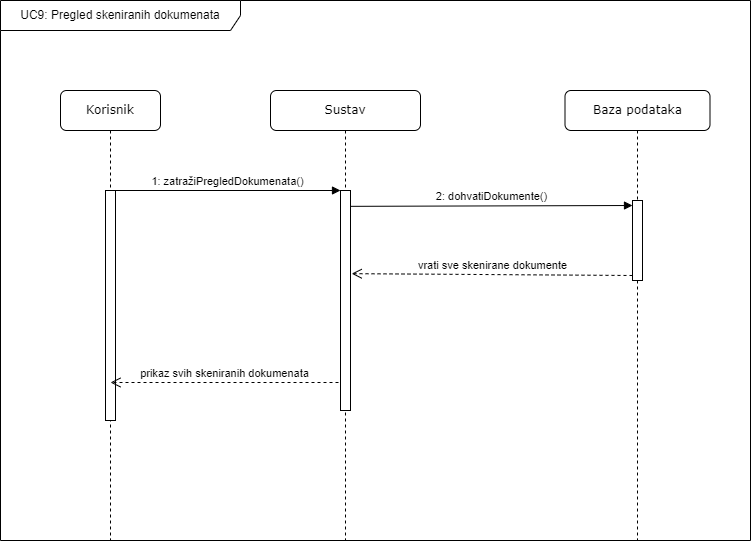
\includegraphics[width=\textwidth]{slike/sekvencijski_dijagram_UC9.PNG} %veličina u odnosu na širinu linije
					\caption{Slika broj: Sekvencijski dijagram za UC9}
					\label{fig:UC9} %label mora biti drugaciji za svaku sliku
				\end{figure}
				\clearpage

				\textbf{Obrazac uporabe UC21 - Digitalizacija dokumenta}\
				
				Korisnik šalje sliku  u sustav koji zatim tu sliiku učitava i pregledava je li na slici dokument. Ako je, onda na njega primjenjuje OCR te novonastali dokument sprema u bazu podataka. Ako na slici nije očitan dokument, sustav korisniku šalje obavijst da učitana slika ne sadrži dokument te mu daje opciju da priloži novu sliku.
				\begin{figure}[H]
					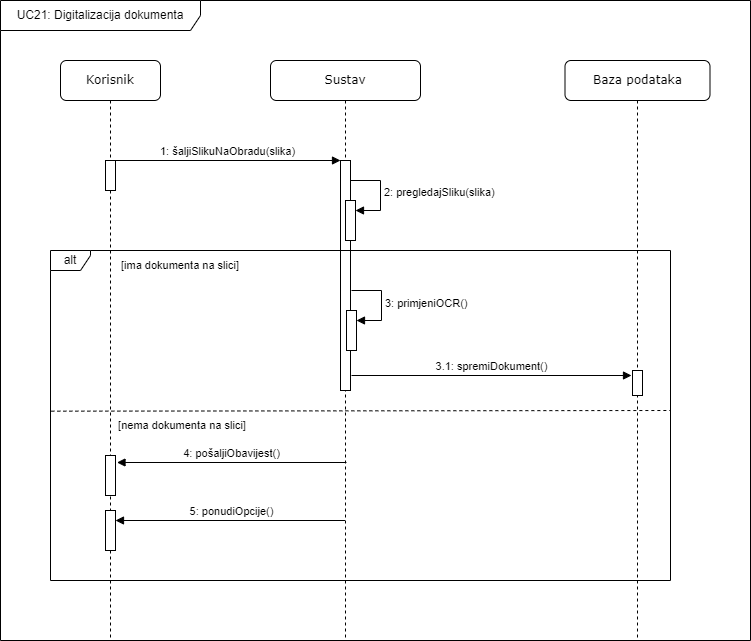
\includegraphics[width=\textwidth]{slike/sekvencijski_dijagram_UC21.PNG} %veličina u odnosu na širinu linije
					\caption{Slika broj: Sekvencijski dijagram za UC21}
					\label{fig:UC21} %label mora biti drugaciji za svaku sliku
				\end{figure}		
				\clearpage

				\eject
	
		\section{Ostali zahtjevi}

			 	\begin{packed_item}
			 	
			 	\item Sustav treba omogućiti rad više korisnika u istom razdoblju
			 	\item Korisničko sučelje ne smije imati greške(bug-ove) kojima je moguće da klijent ima pristup ovlastima koje mu ne bi trebale biti dozvoljene
			 	\item Sustav treba biti implementiran kao mobilna aplikacija koja koristeći objektno-orijentirane jezike
			 	\item Korisničko sučelje treba biti u stanju podržavati različite dijakritičke znakove u tekstualnom sučelju
			 	\item Dohvaćanje podataka iz baze podataka i njihov prikaz ne smije trajati duže od nekoliko sekundi
			 	\item Veza s bazom mora biti sigurna i zaštićena kako bi bila otporna na krađu klasificiranih podataka tvrtke
			 	\item Sustav treba imati intuitivno i jednostavno korisničko sučelje za koje nisu potrebne upute korištenja
			 	\item Eventualna nadogradnja sustava ne smije brisati značajke aplikacije protiv volje korisnika aplikacije
			 		
			 	\end{packed_item}
			 
			 
			 
	